% !TeX program = xelatex

\documentclass[
    a4paper,
    14pt,
    twoside,
]{extarticle}

% -- document classes --
\usepackage{extsizes}

% -- embed other PDFs --
\usepackage{pdfpages}

% -- fonts and encoding --
\usepackage[utf8]{inputenc}
\usepackage[T2A]{fontenc}

\usepackage[
    english,
    russian,
]{babel}
\usepackage{csquotes}

\usepackage{fontspec}
\setmainfont{Times New Roman}

% -- margins --
\usepackage[
    left=30mm,
    right=10mm,
    top=20mm,
    bottom=20mm,
    nohead,
    includefoot,
    footskip=10mm,
]{geometry}

% -- spacing --
\usepackage{setspace}
\onehalfspacing

% -- indentation --
\usepackage{indentfirst}
\setlength\parindent{1.25cm}

% -- titles --
\usepackage{titlesec}

\titleformat{\section}
    {\fontsize{18}{18}\bfseries}
    {\thesection.}
    {0.5em}
    {\centering}

\titleformat{\subsection}
    {\fontsize{16}{16}\bfseries}
    {\thesubsection.}
    {0.5em}
    {\centering}

\titleformat{\subsubsection}
    {\fontsize{14}{14}\itshape}
    {\thesubsubsection.}
    {0.5em}
    {\centering}

% -- table of contents --
\addto\captionsrussian{\renewcommand{\contentsname}{СОДЕРЖАНИЕ}}

\usepackage{tocloft}

\renewcommand{\cfttoctitlefont}{\hfil\fontsize{18}{18}\bfseries}
\renewcommand{\cftaftertoctitle}{\hfil}

\renewcommand{\cftsecfont}{\normalfont}
\renewcommand{\cftsecpagefont}{\normalfont}
\renewcommand{\cftsecleader}{\cftdotfill{\cftdotsep}}
\renewcommand{\cftsecaftersnum}{.}
\renewcommand{\cftbeforesecskip}{0em}
\renewcommand{\cftsecnumwidth}{2em}

\renewcommand{\cftsubsecfont}{\normalfont}
\renewcommand{\cftsubsecpagefont}{\normalfont}
\renewcommand{\cftsubsecleader}{\cftdotfill{\cftdotsep}}
\renewcommand{\cftsubsecaftersnum}{.}
\renewcommand{\cftbeforesubsecskip}{0em}
\renewcommand{\cftsubsecnumwidth}{2.7em}

\renewcommand{\cftsubsubsecfont}{\normalfont}
\renewcommand{\cftsubsubsecpagefont}{\normalfont}
\renewcommand{\cftsubsubsecleader}{\cftdotfill{\cftdotsep}}
\renewcommand{\cftsubsubsecaftersnum}{.}
\renewcommand{\cftbeforesubsubsecskip}{0em}
\renewcommand{\cftsubsubsecnumwidth}{4em}

% -- figures --
\usepackage{graphicx}
\usepackage{float}

\usepackage[
    font=small,
    labelsep=endash,
]{caption}
\captionsetup[table]{singlelinecheck=off}

\addto\captionsrussian{\renewcommand{\figurename}{Рисунок}}

% -- tables --
\usepackage{booktabs}

\usepackage{tabularx}
\usepackage{xltabular}

\usepackage{ltablex}
\keepXColumns

\usepackage{multirow}

\usepackage[table]{xcolor}
\usepackage{colortbl}
\definecolor{table-gray}{gray}{0.5}
\definecolor{table-lightgray}{gray}{0.75}

% -- math --
\usepackage{amsmath}
\usepackage{amsfonts}
\usepackage{amsthm}
\usepackage{mathtools}
\usepackage{physics}
\usepackage{interval}
\usepackage{bm}

% -- hyperlinks --
% !!! toc hyperref does NOT work !!!
\usepackage[
    colorlinks=false,
    unicode=true,
    hidelinks=true,
    bookmarks,
    hypertexnames=false,
    % draft,
]{hyperref}

% \usepackage{bookmarks}
\usepackage{bookmark}

% -- bibliography --
\usepackage[
    backend=biber,
    natbib=true,
    style=gost-numeric,
    defernumbers=true,
]{biblatex}

\setlength\bibparsep{0em}

% -- misc --
\sloppy

\usepackage{pdflscape}

\usepackage{enumitem}
\setlist{nosep}

\newcommand{\Item}{\item[\textbullet]}

% -- other --
\usepackage{lipsum}


\begin{document}

\begin{titlepage}

  \begin{center}
    НАЦИОНАЛЬНЫЙ ИССЛЕДОВАТЕЛЬСКИЙ УНИВЕРСИТЕТ ИТМО\\[0.1cm]
    Факультет инфокоммуникационных технологий\\
    Инфокоммуникационные технологии и системы связи\\[5cm]

    {\Large Лабораторная работа №3}\\[0.1cm]
    \noindent<<Формализация требований>>\\[3cm]
  \end{center}

  \begin{minipage}{0.65\linewidth}
    \hspace{\fill}
  \end{minipage}
  \begin{minipage}{0.25\linewidth}
    Выполнил:\\
    Савчук А. А.\\
    Группа К4112с \\

    Проверил:\\
    Марченко Е. В.
  \end{minipage}

  \vfill

  \begin{center}
    Санкт-Петербург\\
    \the\year
  \end{center}

\end{titlepage}

\setcounter{page}{2}

\tableofcontents

\newpage
\section*{\MakeUppercase{Введение}}\label{sec:introduction}
\addcontentsline{toc}{section}{Введение}
Цель работы -- ознакомиться с методологией построения диаграмм потоков данных.


\newpage
\section{Требования на создание системы}
\subsection*{Вариант задания}

Электронная система продажи билетов на междугородние маршруты.

\subsection*{Описание инфокоммуникационной системы}

Платформа для продажи электронных билетов на междугородние автобусные поездки и
получения онлайн-платежей за проезд. Покупатель самостоятельно распечатывает
билеты для предъявления перед отправкой. Оплатить билет можно из-за рубежа РФ.
Доступна покупка поездок <<туда-обратно>>, включая пересадки и использование
абонементов. Обновление таблиц в режиме реального времени.

Реализация проездных документов для людей с ограниченными возможностями не
требует посещения кассы: средства можно перевести на выбор через SMS,
электронные кошельки или банковские карты. Данные электронных расчетов
интегрированы с бухгалтерией компании.

\subsection{Концепция проекта}

\textbf{Для} пассажиров междугородних автобусов,
\textbf{которые} хотят иметь возможность
просмотра доступных маршрутов в режиме реального времени,
покупки билетов с помощью компьютера или мобильного телефона,
используя различные способы оплаты,
\textbf{а также для} пассажиров междугородних автобусов с особыми потребностями,
\textbf{которые} имеют трудности с посещением кассы
при покупке билетов на междугородние автобусные маршруты и хотят иметь
возможность покупки билетов онлайн,
\textbf{эта} инфокоммуникационная система
\textbf{является} электронной системой
продажи билетов на междугородние маршруты,
\textbf{которая} позволяет
просматривать доступные междугородние автобусные
маршруты в режиме реального времени,
покупать билеты с помощью компьютера или мобильного телефона,
использовать различные способы оплаты при покупке билетов (через SMS,
электронные кошельки или банковские карты), а также использовать абонементы.
покупать билеты <<туда-обратно>> и с пересадками,
покупать билеты из-за рубежа РФ.
\textbf{В отличие от} традиционного способа продажи билетов, требующего
от пассажира личного посещения кассы,
\textbf{наш продукт} позволяет покупать билеты на междугородние автобусные
маршруты онлайн с помощью компьютера или мобильного телефона.

\subsection{Пользователи системы}

Выделим следующие классы пользователей: конечные пользователи, корпоративные
клиенты, администраторы.

\subsubsection*{Конечные пользователи}

Это пользователи, которые непосредственно используют систему для поиска и
покупки билетов на междугородние автобусы. Класс содержит единственный тип
\textit{пассажиры междугородних автобусных маршрутов}, который включает
следующие роли.

\null

\noindent\textit{Пользователь-гость}

\noindent цели:
\begin{itemize}
    \item быстро найти доступные маршруты и узнать стоимость билетов без
    необходимости регистрации;
    \item получить общую информацию о поездках и доступных вариантах.
\end{itemize}

\noindent ожидания:
\begin{itemize}
    \item удобный и быстрый интерфейс для поиска маршрутов;
    \item минимум шагов для поиска информации;
    \item возможность легко зарегистрироваться для покупки билета.
\end{itemize}

\null

\noindent\textit{Рядовой пользователь}

\noindent цели:
\begin{itemize}
    \item купить билет на нужный маршрут быстро и удобно;
    \item иметь возможность сохранять свои данные для упрощения
    последующих покупок.
\end{itemize}

\noindent ожидания:
\begin{itemize}
    \item персонализированный опыт: сохраненные маршруты, пассажиры,
    история поездок;
    \item удобная система оплаты и быстрая обработка транзакций;
    \item поддержка разных способов оплаты.
\end{itemize}

\null

\noindent\textit{Пользователь с особыми потребностями}

\noindent цели:
\begin{itemize}
    \item купить билет на нужный маршрут без необходимости посещать
    кассу;
    \item получить доступ к адаптированной системе с улучшенной
    доступностью.
\end{itemize}

\noindent ожидания:
\begin{itemize}
    \item удобный интерфейс для самостоятельной покупки билета онлайн;
    \item настраиваемая цветовая схема и крупные элементы интерфейса;
    \item возможность переключения на более доступные версии сайта;
    \item поддержка специальных возможностей, таких как озвучивание
    текста.
\end{itemize}

\null

\noindent\textit{Иностранный пользователь}

\noindent цели:
\begin{itemize}
    \item легко пользоваться системой на понятном языке;
    \item купить билет на поездку быстро и удобно.
\end{itemize}

\noindent ожидания:
\begin{itemize}
    \item поддержка нескольких языков, включая перевод интерфейса и
    инструкций;
    \item возможность оплаты в валюте или с использованием международных
    платёжных систем.
\end{itemize}

\subsubsection*{Корпоративные клиенты}

Это компании, предоставляющие услуги междугородних автобусных перевозок и
использующие систему для автоматизации учета транзакций. Класс содержит
единственный тип \textit{компании-организаторы междугородних автобусных
перевозок}, который включает единственную роль.

\null

\noindent\textit{Автоматизированная система бухгалтерского учета}

\noindent цели:
\begin{itemize}
    \item получать данные о транзакциях за билеты для автоматической
    обработки;
    \item интегрировать систему оплаты с 1C:Бухгалтерия для облегчения
    учёта.
\end{itemize}

\noindent ожидания:
\begin{itemize}
    \item простая и нативная интеграция с REST API 1C:Бухгалтерия без
    сложных дополнительных настроек;
    \item возможность выбора между выгрузкой данных в режиме реального
    времени или по расписанию;
    \item полная автоматизация процессов бухгалтерского учёта с
    минимальными затратами на интеграцию.
\end{itemize}

\subsubsection*{Администраторы}

Это пользователи, которые управляют и поддерживают
работоспособность системы, а также редактируют контент, связанный с расписаниями
и другими данными. Класс содержит следующие типы и роли:
\begin{itemize}
    \item (тип) технические администраторы -- (роль) системный администратор;
    \item (тип) контент-администраторы -- (роль) модератор расписаний.
\end{itemize}

\null

\noindent\textit{Системный администратор}

\noindent цели:
\begin{itemize}
    \item эффективное управление учетными записями пользователей;
\end{itemize}

\noindent ожидания:
\begin{itemize}
    \item доступ к интерфейсу для создания, редактирования, блокировки и
    удаления учетных записей;
    \item возможность сброса паролей;
\end{itemize}

\null

\noindent\textit{Модератор расписаний}

\noindent цели:
\begin{itemize}
    \item управление расписаниями автобусных маршрутов;
    \item обеспечение актуальности и корректности информации о рейсах.
\end{itemize}

\noindent ожидания:
\begin{itemize}
    \item доступ к интерфейсу для добавления, изменения и удаления
    расписаний маршрутов;
    \item возможность быстро вносить коррективы при изменениях в
    маршрутах или расписаниях.
\end{itemize}

\subsection{Пользовательские истории}

\subsubsection*{Пользователь-гость}
\begin{itemize}
    \item Как пользователь-гость, я хочу быстро найти доступные маршруты и узнать стоимость билетов, чтобы получить информацию без регистрации.
    \item Как пользователь-гость, я хочу легко зарегистрироваться при необходимости, чтобы иметь возможность покупать билеты онлайн.
\end{itemize}

\subsubsection*{Рядовой пользователь}
\begin{itemize}
    \item Как рядовой пользователь, я хочу купить билет на нужный маршрут, чтобы сэкономить время и избежать очередей.
    \item Как рядовой пользователь, я хочу сохранить свои данные для последующих покупок, чтобы процесс был более быстрым.
    \item Как рядовой пользователь, я хочу оплачивать билет разными способами (банковская карта, СБП, SMS, электронный кошелек), чтобы выбрать наиболее удобный вариант оплаты.
    \item Как рядовой пользователь, я хочу, чтобы после покупки билета в мой календарь автоматически добавлялось событие-напоминание о поездке, чтобы не забыть о времени отправления.
\end{itemize}

\subsubsection*{Пользователь с особыми потребностями}
\begin{itemize}
    \item Как пользователь с особыми потребностями, я хочу купить билет без посещения кассы, чтобы упростить процесс покупки.
    \item Как пользователь с особыми потребностями, я хочу воспользоваться адаптированной системой с улучшенной доступностью, чтобы комфортно использовать все функции системы.
\end{itemize}

\subsubsection*{Иностранный пользователь}
\begin{itemize}
    \item Как иностранный пользователь, я хочу выбрать удобный для меня язык интерфейса, чтобы пользоваться системой без языковых барьеров.
    \item Как иностранный пользователь, я хочу оплатить билет с помощью международных платежных систем, чтобы покупка была возможна независимо от валюты.
\end{itemize}

\subsubsection*{Автоматизированная система бухгалтерского учета}
\begin{itemize}
    \item Как автоматизированная система бухгалтерского учета, я хочу получать данные о транзакциях в режиме реального времени или по расписанию, чтобы они автоматически обрабатывались.
    \item Как автоматизированная система бухгалтерского учета, я хочу простую и нативную интеграцию с 1C:Бухгалтерия, чтобы минимизировать затраты на настройку.
\end{itemize}

\subsubsection*{Системный администратор}
\begin{itemize}
    \item Как системный администратор, я хочу иметь доступ к интерфейсу для управления учетными записями, чтобы создавать, редактировать, блокировать и удалять учетные записи пользователей.
    \item Как системный администратор, я хочу возможность сброса паролей, чтобы помогать пользователям восстанавливать доступ к своим учетным записям.
\end{itemize}

\subsubsection*{Модератор расписаний}
\begin{itemize}
    \item Как модератор расписаний, я хочу управлять расписаниями маршрутов, чтобы поддерживать их актуальность и корректность.
    \item Как модератор расписаний, я хочу быстро вносить изменения в расписания, чтобы оперативно реагировать на изменения в рейсах.
\end{itemize}

\subsection{Функциональные требования}

Функциональные требования к системе и соответствующие им задачи разработчика
приведены в таблице \ref{table-req} в приложении \hyperref[appendix-1]{А}.


\section{Функциональная модель}
\subsection{Контекстная диаграмма}

\begin{figure}[H]
    \centering
    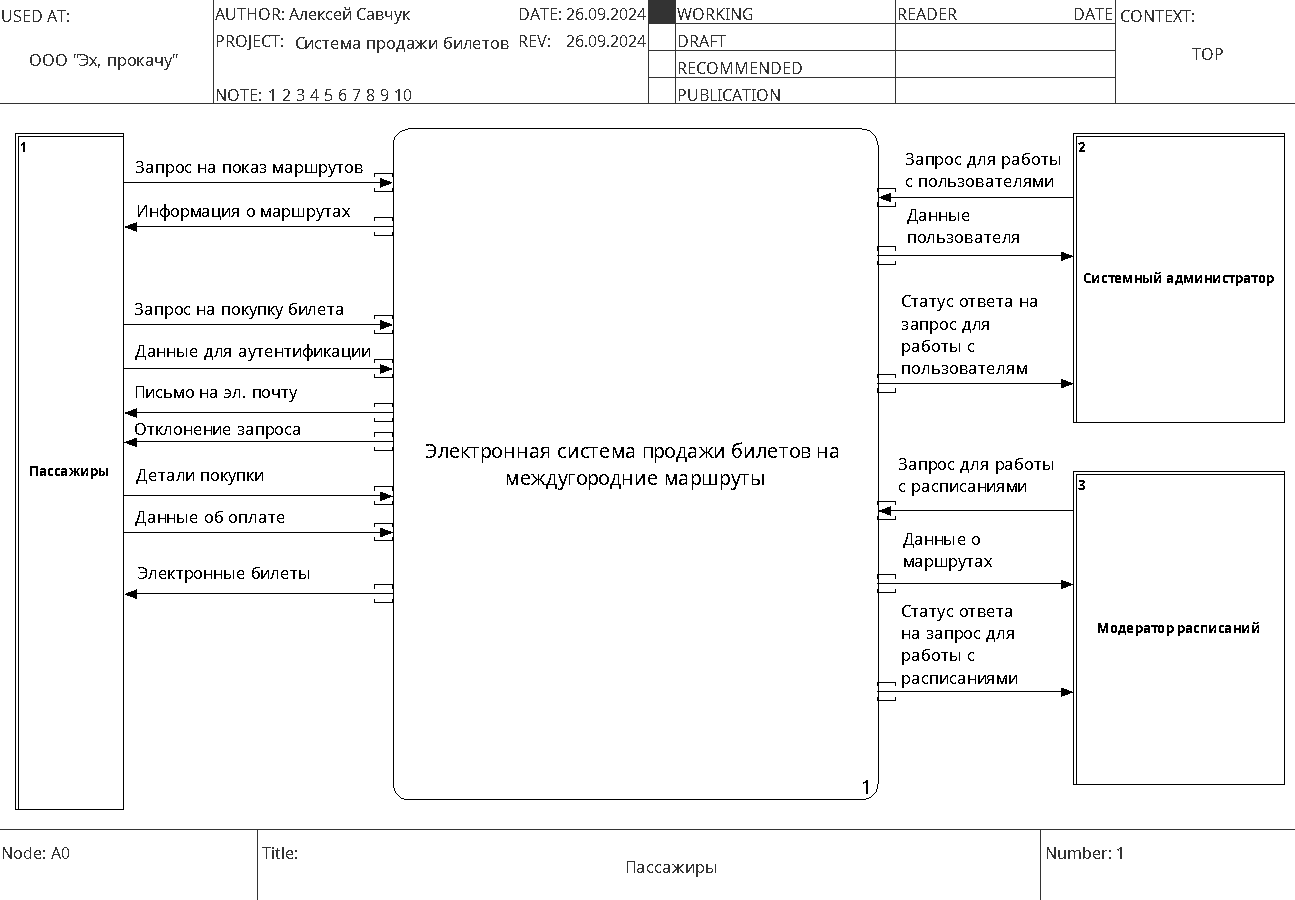
\includegraphics[width=\linewidth]{model/A0.png}
    \caption{Контекстная диаграмма}
\end{figure}

\newpage
\subsection{Диаграмма декомпозиции 1-го уровня}

\begin{figure}[H]
    \centering
    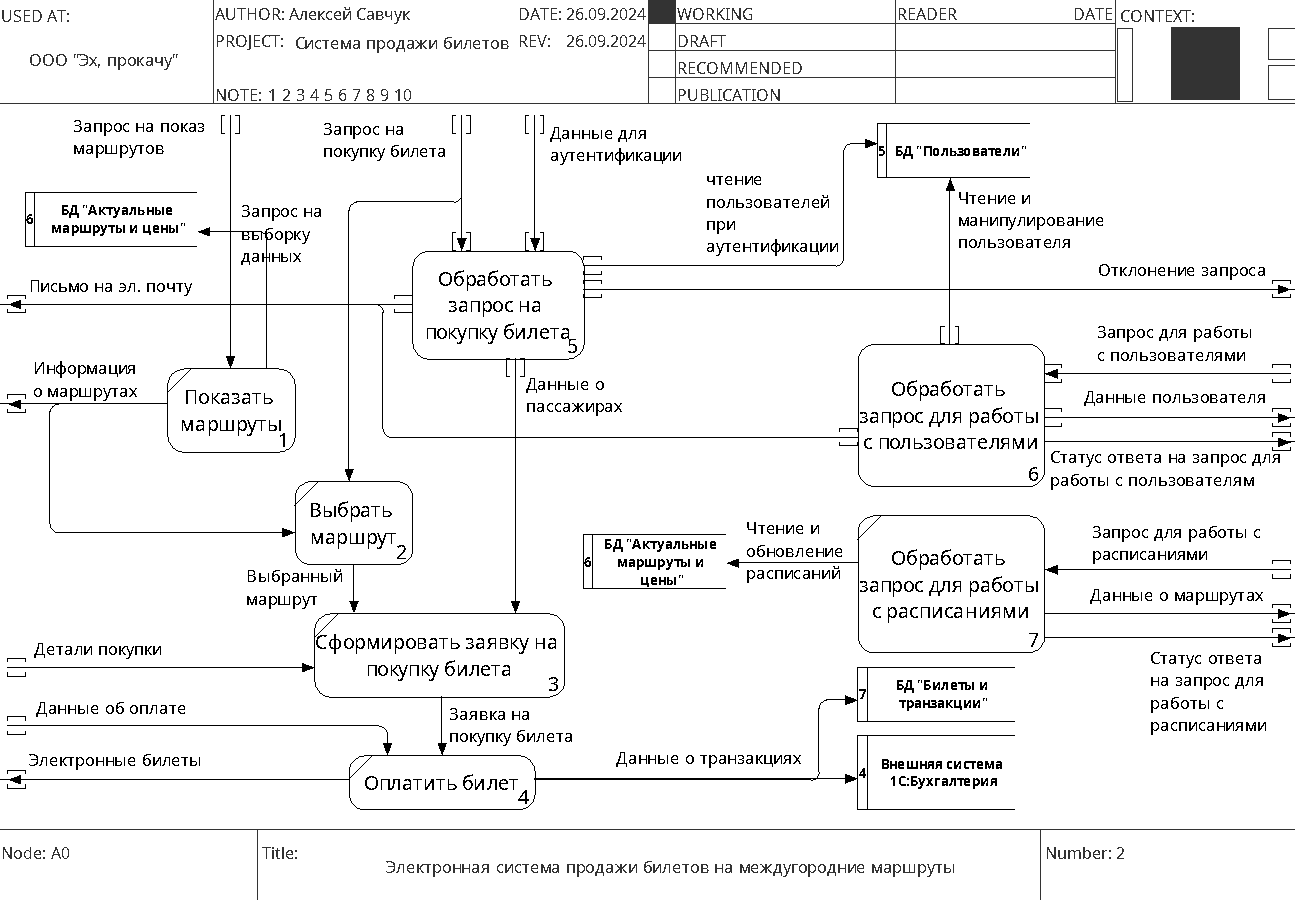
\includegraphics[width=\linewidth]{model/A1.png}
    \caption{Диаграмма декомпозиции 1-го уровня}
\end{figure}

\newpage
\subsection{Диаграммы декомпозиции 2-го уровня}

\begin{figure}[H]
    \centering
    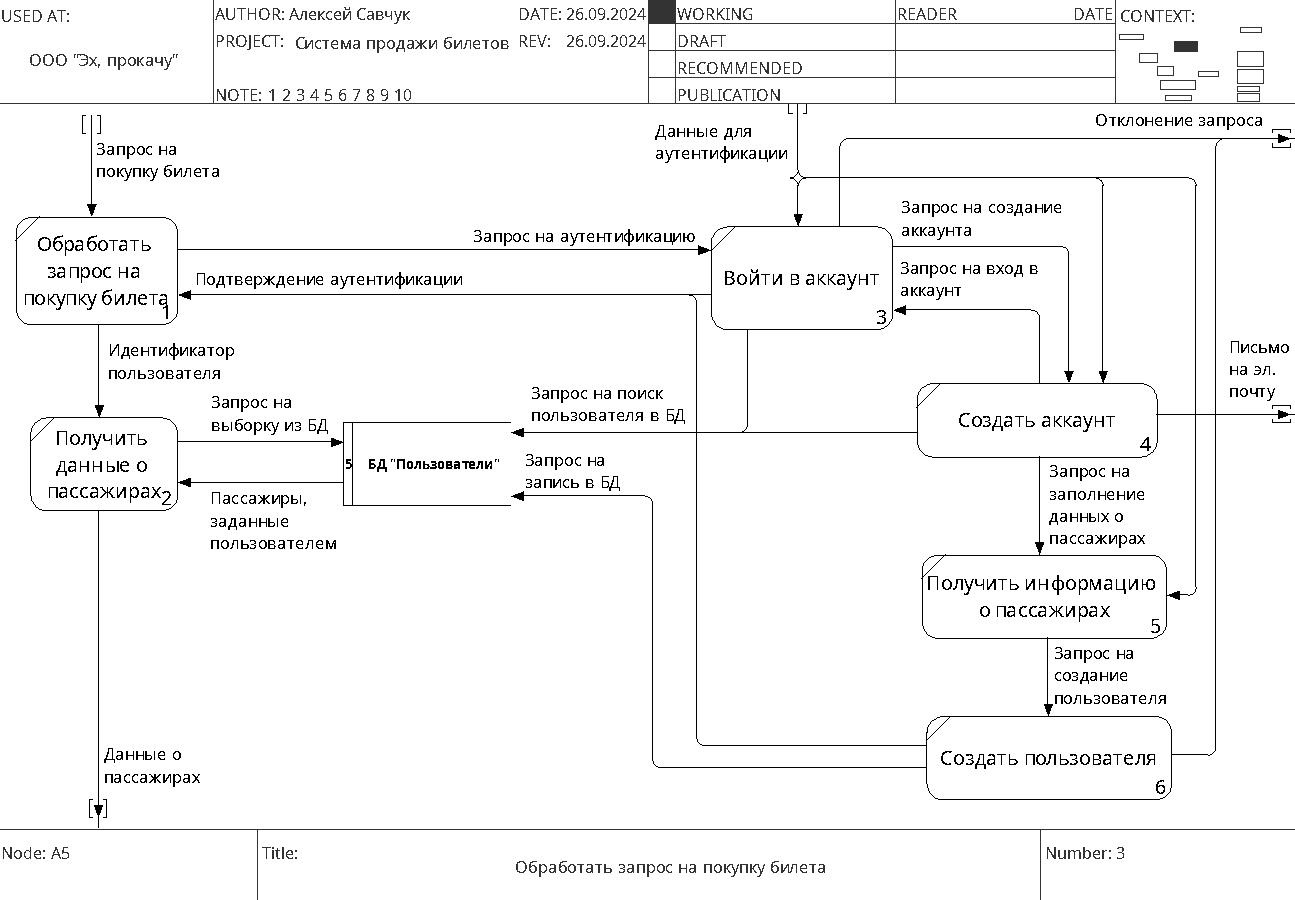
\includegraphics[width=\linewidth]{model/A2-1.png}
    \caption{Диаграмма декомпозиции 2-го уровня: аутентификация}
\end{figure}

\newpage
\begin{figure}[H]
    \centering
    \includegraphics[width=\linewidth]{model/A2-2.png}
    \caption{Диаграмма декомпозиции 2-го уровня: создание заявки на покупку билета}
\end{figure}


\newpage
\section*{\MakeUppercase{Заключение}}\label{sec:conclusion}
\addcontentsline{toc}{section}{Заключение}
В рамках данной работы для разработанной ранее диаграммы классы были реализованы
классы с применением шаблонов проектирования GoF (Gang of Four), что позволило
улучшить архитектуру системы, обеспечив гибкость, расширяемость и повторное использование
компонентов.

\newpage
\section*{Приложение А}\label{appendix-1}
\addcontentsline{toc}{section}{Приложение А}

\setcounter{table}{0}
\renewcommand{\thetable}{A.\arabic{table}}
\newcounter{ReqID}
\newcounter{TaskID}

\newcommand{\ReqID}{
    \stepcounter{ReqID}
    \setcounter{TaskID}{0}
    \arabic{ReqID}
}
\newcommand{\TaskID}{
    \stepcounter{TaskID}
    \arabic{ReqID}.\arabic{TaskID}
}

\newcommand{\Req}[1]{%
    \multirow[t]{100}{=}{\ReqID} &%
    \multirow[t]{100}{=}{#1}%
}
\newcommand{\ReqStub}{&}
\newcommand{\Task}[1]{\TaskID & {#1}}
\newcommand{\ReqTaskStub}{& & &}

{
    \centering
    \fontsize{12}{14}\selectfont
    \begin{xltabular}{\linewidth}
    {
        |>{\hsize=.1\hsize\linewidth=\hsize}X
        |>{\hsize=.4 \hsize\linewidth=\hsize}X
        |>{\hsize=.1\hsize\linewidth=\hsize}X
        |>{\hsize=.4 \hsize\linewidth=\hsize}X|
    }
        \caption{Функциональные требования}\label{table-req}\\
        \hline
        \rowcolor{table-gray}
        \textcolor{white}{\textbf{ID}} & \textcolor{white}{\textbf{Описание <<рамки решения>>}} &
        \textcolor{white}{\textbf{ID}} & \textcolor{white}{\textbf{Описание <<рамки проекта>>}} \\
        \hline
        \endfirsthead

        \caption*{Продолжение таблицы \ref{table-req}}\\
        \hline
        \rowcolor{table-gray}
        \textcolor{white}{\textbf{ID}} & \textcolor{white}{\textbf{Описание <<рамки решения>>}} &
        \textcolor{white}{\textbf{ID}} & \textcolor{white}{\textbf{Описание <<рамки проекта>>}} \\
        \hline
        \endhead


        \rowcolor{table-lightgray}
        \multicolumn{4}{|l|}{
            \textbf{Просмотр доступных междугородних автобусных маршрутов}
        } \\
        \hline

        % DONE
        \Req{%
            % На главной странице приложения доступна форма поиска маршрутов со
            % следующими полями выбора: начальный и конечный пункт маршрута, дата
            % поездки.
            Система должна отображать на главной странице форму поиска маршрутов
            с полями для выбора начального и конечного пунктов, а также даты
            поездки.
        } & \Task{
            Добавить форму поиска маршрутов на главную страницу.
        } \\
        \cline{3-4}
        \ReqStub & \Task{
            Включить поля: начальный пункт, конечный пункт и дата поездки.
        } \\
        \cline{3-4}
        \ReqStub & \Task{
            Сделать так, чтобы форма появлялась при открытии главной страницы.
        } \\
        \ReqTaskStub \\
        \ReqTaskStub \\
        \hline

        % DONE
        \Req{%
            % Форма поиска маршрутов должна быть доступна для всех пользователей:
            % как авторизированных, так и неавторизированных.
            Система должна предоставлять форму поиска маршрутов на главной
            странице приложения для всех пользователей, независимо от статуса
            авторизации.
        } & \Task{
            Сделать форму поиска доступной для всех пользователей.
        } \\
        \cline{3-4}
        \ReqStub & \Task{
            Протестировать, что форма работает одинаково для авторизованных и
            неавторизованных пользователей.
        } \\
        \hline

        % DONE
        \Req{%
            % Выбор начального и конечного пункта маршрута осуществляется из
            % конечного числа предопределенных вариантов.
            Система должна предоставлять пользователю возможность выбора
            начального и конечного пунктов маршрута из заранее определенного
            списка вариантов.
        } & \Task{
            Создать список предопределенных пунктов для выбора маршрута.
        } \\
        \cline{3-4}
        \ReqStub & \Task{
            Добавить возможность выбора пунктов из этого списка в форме поиска.
        } \\
        \ReqTaskStub \\
        \hline

        % DONE
        \Req{%
            % При выборе начального и конечного пункта маршрута доступен поиск во
            % множестве предопределенных вариантов.
            Система должна обеспечивать возможность поиска среди
            предопределенных вариантов при выборе начального и конечного пунктов
            маршрута.
        } & \Task{
            Реализовать поиск по списку предопределенных пунктов в форме выбора
            начального и конечного маршрута.
        } \\
        \cline{3-4}
        \ReqStub & \Task{
            Настроить отображение результатов поиска при вводе данных
            пользователем.
        } \\
        \ReqTaskStub \\
        \ReqTaskStub \\
        \ReqTaskStub \\
        \ReqTaskStub \\
        \hline

        % DONE
        \Req{%
            % Поиск при выборе начального и конечного пункта маршрута должен быть
            % \textit{нечётким поиском}.
            Система должна поддерживать \textit{нечёткий поиск} при выборе
            начального и конечного пункта маршрута из предопределенных
            вариантов.
        } & \Task{
            Реализовать механизм нечёткого поиска для выбора начального и
            конечного пунктов маршрута.
        } \\
        \cline{3-4}
        \ReqStub & \Task{
            Обеспечить корректное отображение результатов нечёткого поиска.
        } \\
        \hline

        % DONE
        \Req{%
            % После выполнения поиска маршрутов пользователь переходит на страницу
            % со списком доступных маршрутов.
            Система должна перенаправлять пользователя на страницу со списком
            доступных маршрутов после выполнения поиска.
        } & \Task{
            Настроить перенаправление на страницу с результатами поиска после
            выбора маршрута.
        } \\
        \cline{3-4}
        \ReqStub & \Task{
            Реализовать отображение списка доступных маршрутов на новой
            странице.
        } \\
        \hline

        % DONE
        \Req{%
            % На странице со списком доступных маршрутов перечислены все маршруты
            % удовлетворяющие условиям поиска, для каждого маршрута показаны его
            % время отправления и прибытия, время в пути, цена за билет в одну
            % сторону и цена за билет в обе стороны.
            Система должна отображать на странице со списком все маршруты,
            соответствующие условиям поиска, с указанием времени отправления,
            прибытия, времени в пути, а также цен на билет в одну и обе стороны.
        } & \Task{
            Реализовать отображение списка маршрутов, соответствующих
            результатам поиска.
        } \\
        \cline{3-4}
        \ReqStub & \Task{
            Добавить к каждому маршруту информацию о времени отправления,
            прибытия, времени в пути и ценах на билеты.
        } \\
        \hline

        % DONE
        \Req{%
            % Маршруты на странице со списком доступных маршрутов сортируются по
            % возрастанию времени отправления.
            Система должна сортировать маршруты на странице со списком доступных
            маршрутов по возрастанию времени отправления.
        } & \Task{
            Настроить сортировку списка маршрутов по возрастанию времени
            отправления.
        } \\
        \cline{3-4}
        \ReqStub & \Task{
            Обеспечить правильное отображение отсортированных маршрутов на
            странице.
        } \\
        \hline

        \rowcolor{table-lightgray}
        \multicolumn{4}{|l|}{
            \textbf{Регистрация нового аккаунта (регистрация)}
        } \\
        \hline

        % DONE
        \Req{%
            % На главной странице приложения доступно действие для перехода на
            % страницу входа в аккаунт/создания нового аккаунта.
            Система должна предоставлять на главной странице действие для
            перехода на страницу входа или создания нового аккаунта.
        } & \Task{
            Добавить кнопку или ссылку на главной странице для перехода на
            страницу входа/регистрации.
        } \\
        \cline{3-4}
        \ReqStub & \Task{
            Настроить переход на соответствующую страницу при нажатии.
        } \\
        \hline

        % DONE
        \Req{%
            % На странице создания нового аккаунта доступна форма создания нового
            % аккаунта со следующими полями: адрес электронной почты, пароль,
            % повторение пароля.
            Система должна предоставлять на странице создания нового аккаунта
            форму с полями для ввода адреса электронной почты, пароля и
            повторения пароля.
        } & \Task{
            Создать форму на странице регистрации с полями для электронной
            почты, пароля и повторения пароля.
        } \\
        \cline{3-4}
        \ReqStub & \Task{
            Настроить отправку данных формы для создания нового аккаунта.
        } \\
        \hline

        % DONE
        \Req{%
            % После успешного заполнения формы на странице создания нового
            % аккаунта пользователь переходит на страницу подтверждения адреса
            % электронной почты, где он должен ввести код из письма, отправленного
            % на указанный адрес электронной почты.
            Система должна перенаправлять пользователя на страницу подтверждения
            адреса электронной почты после успешного заполнения формы создания
            нового аккаунта, где пользователь должен ввести код из письма,
            отправленного на указанный адрес.
        } & \Task{
            Настроить перенаправление на страницу подтверждения электронной
            почты после успешной регистрации.
        } \\
        \cline{3-4}
        \ReqStub & \Task{
            Реализовать форму для ввода кода подтверждения на странице
            подтверждения.
        } \\
        \cline{3-4}
        \ReqStub & \Task{
            Сгенерировать код подтверждения при создании нового аккаунта.
        } \\
        \ReqStub & \Task{
            Отправить письмо с кодом подтверждения на указанный адрес
            электронной почты.
        } \\
        \hline

        % DONE
        \Req{%
            % После успешного подтверждения адреса электронной почты пользователь
            % переходит на страницу для заполнения данных о пассажире, включая
            % следующие данные: фамилия, имя, отчество (при наличии), дата
            % рождения, данные паспорта.
            Система должна перенаправлять пользователя на страницу для ввода
            данных о пассажире после успешного подтверждения адреса электронной
            почты. На странице должны быть поля для фамилии, имени, отчества
            (при наличии), даты рождения и данных паспорта.
        } & \Task{
            Настроить перенаправление на страницу ввода данных о пассажире после
            подтверждения электронной почты.
        } \\
        \cline{3-4}
        \ReqStub & \Task{
            Создать форму для ввода данных о пассажире: фамилия, имя, отчество
            (опционально), дата рождения, данные паспорта.
        } \\
        \cline{3-4}
        \ReqStub & \Task{
            Обеспечить корректную отправку данных формы для дальнейшей
            обработки.
        } \\
        \hline

        % DONE
        \Req{%
            % После успешного заполнения данных о пассажире пользователь переходит
            % на главную страницу или, если пользователь создал новый аккаунт
            % после выбора маршрута для покупки билета, на страницу покупки билета
            % для выбранного ранее маршрута.
            Система должна перенаправлять пользователя на главную страницу после
            успешного заполнения данных о пассажире. Если новый аккаунт был
            создан после выбора маршрута для покупки билета, система должна
            перенаправить пользователя на страницу покупки билета для выбранного
            маршрута.
        } & \Task{
            Настроить перенаправление на главную страницу после успешного
            заполнения данных о пассажире.
        } \\
        \cline{3-4}
        \ReqStub & \Task{
            Реализовать логику перенаправления на страницу покупки билета, если
            регистрация произошла после выбора маршрута.
        } \\
        \ReqTaskStub \\
        \ReqTaskStub \\
        \ReqTaskStub \\
        \ReqTaskStub \\
        \ReqTaskStub \\
        \hline

        \rowcolor{table-lightgray}
        \multicolumn{4}{|l|}{
            \textbf{Вход в аккаунт пользователя (аутентификация)}
        } \\
        \hline

        % DONE
        \Req{%
            % На странице создания входа в аккаунт доступна форма со следующими
            % полями: адрес электронной почты, пароль.
            Система должна предоставлять на странице входа в аккаунт форму с
            полями для ввода адреса электронной почты и пароля.
        } & \Task{
            Создать форму на странице входа с полями для электронной почты и
            пароля.
        } \\
        \cline{3-4}
        \ReqStub & \Task{
            Настроить отправку данных формы для проверки учетных данных
            пользователя.
        } \\
        \hline

        % DONE
        \Req{%
            % После успешного заполнения формы на странице входа в аккаунт
            % пользователь переходит на главную страницу или, если пользователь
            % вошел в аккаунт после выбора маршрута для покупки билета, на
            % страницу покупки билета для выбранного ранее маршрута.
            Система должна перенаправлять пользователя на главную страницу после
            успешного входа в аккаунт. Если вход был выполнен после выбора
            маршрута для покупки билета, пользователь должен быть перенаправлен
            на страницу покупки билета для выбранного маршрута.
        } & \Task{
            Настроить перенаправление на главную страницу после успешного входа
            в аккаунт.
        } \\
        \cline{3-4}
        \ReqStub & \Task{
            Реализовать логику перенаправления на страницу покупки билета, если
            вход был выполнен после выбора маршрута.
        } \\
        \ReqTaskStub \\
        \ReqTaskStub \\
        \ReqTaskStub \\
        \hline

        \rowcolor{table-lightgray}
        \multicolumn{4}{|l|}{
            \textbf{Личный кабинет пользователя}
        } \\
        \hline

        % DONE
        \Req{%
            % В личном кабинете пользователя доступно действия для перехода на
            % страницу со списком указанных ранее пользователем пассажиров.
            Система должна предоставлять в личном кабинете пользователя действие
            для перехода на страницу со списком пассажиров, указанных ранее
            пользователем.
        } & \Task{
            Добавить ссылку или кнопку в личном кабинете для перехода на
            страницу со списком пассажиров.
        } \\
        \cline{3-4}
        \ReqStub & \Task{
            Настроить перенаправление на страницу со списком пассажиров при
            нажатии на элемент.
        } \\
        \hline

        % DONE
        \Req{%
            % На странице со списком указанных пассажиров доступно действие для
            % перехода на страницу редактирования данных существующего пассажира.
            Система должна предоставлять на странице со списком пассажиров
            действие для перехода на страницу редактирования данных
            существующего пассажира.
        } & \Task{
            Добавить ссылку или кнопку рядом с каждым пассажиром для перехода на
            страницу редактирования.
        } \\
        \cline{3-4}
        \ReqStub & \Task{
            Настроить перенаправление на страницу редактирования при нажатии на
            элемент.
        } \\
        \hline

        % DONE
        \Req{%
            % На странице со списком указанных пассажиров доступно действие для
            % перехода на страницу добавления нового пассажира.
            Система должна предоставлять на странице со списком пассажиров
            действие для перехода на страницу добавления нового пассажира.
        } & \Task{
            Добавить ссылку или кнопку для перехода на страницу добавления нового пассажира.
        } \\
        \cline{3-4}
        \ReqStub & \Task{
            Настроить перенаправление на страницу добавления пассажира при
            нажатии на элемент.
        } \\
        \hline

        \rowcolor{table-lightgray}
        \multicolumn{4}{|l|}{
            \textbf{Выбор маршрута для покупки билета}
        } \\
        \hline

        % DONE
        \Req{%
            % При выборе маршрута на странице со списком доступных маршрутов,
            % пользователь переходит на страницу покупки билета. При этом если
            % пользователь не авторизован в системе, то он будет перенаправлен на
            % страницу входа в аккаунт/создания нового аккаунта.
            Система должна перенаправлять пользователя на страницу покупки
            билета при выборе маршрута на странице со списком доступных
            маршрутов. Если пользователь не авторизован, он должен быть
            перенаправлен на страницу входа в аккаунт или создания нового
            аккаунта.
        } & \Task{
            Настроить перенаправление на страницу покупки билета при выборе
            маршрута.
        } \\
        \cline{3-4}
        \ReqStub & \Task{
            Реализовать проверку авторизации пользователя перед перенаправлением
            и, при необходимости, перенаправить на страницу входа или
            регистрации.
        } \\
        \ReqTaskStub \\
        \hline

        % DONE
        \Req{%
            % Если после выбора маршрута пользователь был перенаправлен на
            % страницу входа в аккаунт, то после успешной авторизации пользователь
            % будет перенаправлен обратно на страницу покупки билета.
            Система должна перенаправлять пользователя на страницу покупки билета
            после успешной авторизации, если он был перенаправлен на страницу входа
            в аккаунт после выбора маршрута.
        } & \Task{
            Настроить перенаправление на страницу покупки билета после успешной
            авторизации пользователя.
        } \\
        \cline{3-4}
        \ReqStub & \Task{
            Хранить информацию о маршруте, выбранном до перенаправления на
            страницу входа, для корректного возврата.
        } \\
        \hline

        \rowcolor{table-lightgray}
        \multicolumn{4}{|l|}{
            \textbf{Покупка билета для выбранного маршрута}
        } \\
        \hline

        % DONE
        \Req{%
            % После успешного выбора маршрута пользователь переходит на страницу
            % покупки билета на выбранных маршрут.
            Система должна перенаправлять пользователя на страницу покупки
            билета после успешного выбора маршрута.
        } & \Task{
            Настроить перенаправление на страницу покупки билета после успешного
            выбора маршрута.
        } \\
        \cline{3-4}
        \ReqStub & \Task{
            Передать данные о выбранном маршруте на страницу покупки билета.
        } \\
        \hline

        % DONE
        \Req{%
            Система должна предоставлять пользователю возможность выбора билета
            в обе стороны при покупке.
        } & \Task{
            Реализовать опцию выбора билета в обе стороны на странице покупки
            билета.
        } \\
        \cline{3-4}
        \ReqStub & \Task{
            Обновить отображение стоимости и информации о маршруте в зависимости
            от выбранного варианта.
        } \\
        \ReqTaskStub \\
        \ReqTaskStub \\
        \ReqTaskStub \\
        \ReqTaskStub \\
        \ReqTaskStub \\
        \ReqTaskStub \\
        \hline

        % DONE
        \Req{%
            % На странице покупки билета на выборанный маршрут пользователю
            % доступен список пассажиров, доступных для выбора. Список доступных
            % пассажиров формируется из списка пасажиров, указанных пользователем
            % при регистрации и после в личном кабинете.
            Система должна отображать на странице покупки билета список
            пассажиров, доступных для выбора, сформированный из списка
            пассажиров, указанных пользователем при регистрации и в личном
            кабинете.
        } & \Task{
            Реализовать отображение списка пассажиров на странице покупки
            билета.
        } \\
        \cline{3-4}
        \ReqStub & \Task{
            Сформировать список доступных пассажиров из данных, введенных
            пользователем при регистрации и в личном кабинете.
        } \\
        \ReqTaskStub \\
        \ReqTaskStub \\
        \ReqTaskStub \\
        \ReqTaskStub \\
        \ReqTaskStub \\
        \hline

        % DONE
        \Req{%
            Система должна поддерживать возможность использования абонементов
            при оплате билетов.
        } & \Task{
            Реализовать проверку и применение абонементов при оформлении
            покупки.
        } \\
        \cline{3-4}
        \ReqStub & \Task{
            Обновить пользовательский интерфейс для ввода информации об
            абонементе и отображения скидок.
        } \\
        \hline

        % DONE
        \Req{%
            % После выбора пассажиров для покупки билетов пользователю будет ещё
            % раз показана информация о выбранном маршруте, общая стоимость
            % билетов для всех пассажиров, а также обязательная форма
            % подтверждения передачи персональных данных во время обработки
            % запроса на покупку билета.
            Система должна показывать пользователю информацию о выбранном
            маршруте, общую стоимость билетов для всех пассажиров, а также форму
            для подтверждения передачи персональных данных после выбора
            пассажиров для покупки билетов.
        } & \Task{
            Реализовать отображение информации о маршруте и стоимости билетов
            после выбора пассажиров.
        } \\
        \cline{3-4}
        \ReqStub & \Task{
            Создать форму для подтверждения передачи персональных данных во
            время обработки запроса на покупку билета.
        } \\
        \ReqTaskStub \\
        \hline

        % DONE
        \Req{%
            % После подтверждения заявки на покупку билета пользователь переходит
            % на страницу оплаты.
            Система должна перенаправлять пользователя на страницу оплаты после
            подтверждения заявки на покупку билета.
        } & \Task{
            Настроить перенаправление на страницу оплаты после успешного
            подтверждения заявки.
        } \\
        \cline{3-4}
        \ReqStub & \Task{
            Обеспечить передачу данных о покупке на страницу оплаты.
        } \\
        \ReqTaskStub \\
        \ReqTaskStub \\
        \ReqTaskStub \\
        \ReqTaskStub \\
        \hline

        % DONE
        \Req{%
            % Время на оплату ограничено и составляет 15 минут, по истечении
            % этого времени, если пользователь не оплатил билет, заявка на
            % покупку будет отменена.
            Система должна ограничивать время на оплату билета 15 минутами. Если
            пользователь не завершил оплату в установленный срок, заявка на
            покупку должна быть автоматически отменена.
        } & \Task{
            Реализовать таймер обратного отсчета на странице оплаты,
            показывающий оставшееся время.
        } \\
        \cline{3-4}
        \ReqStub & \Task{
            Настроить логику автоматической отмены заявки на покупку по
            истечении 15 минут.
        } \\
        \ReqTaskStub \\
        \hline

        % DONE
        \Req{%
            % На странице оплаты билета пользователю доступен список различных
            % способов оплаты: банковская карта, СБП, SMS, электронный кошелек.
            Система должна предоставлять на странице оплаты билета список
            доступных способов оплаты: банковская карта, СБП, SMS и электронный
            кошелек.
        } & \Task{
            Реализовать отображение списка способов оплаты на странице оплаты
            билета.
        } \\
        \cline{3-4}
        \ReqStub & \Task{
            Настроить функциональность для выбора и обработки каждого способа
            оплаты.
        } \\
        \hline

        % DONE
        \Req{%
            % После успешной оплаты сформированный билет будет отправлен на
            % электронную почту пользователя, а также будет доступен в личном
            % кабинете пользователя.
            Система должна отправлять сформированный билет на электронную почту
            пользователя после успешной оплаты, а также делать его доступным в
            личном кабинете пользователя.
        } & \Task{
            Реализовать отправку билета на электронную почту пользователя после
            подтверждения оплаты.
        } \\
        \cline{3-4}
        \ReqStub & \Task{
            Обеспечить отображение купленного билета в личном кабинете
            пользователя.
        } \\
        \ReqTaskStub \\
        \ReqTaskStub \\
        \ReqTaskStub \\
        \ReqTaskStub \\
        \hline

        % DONE
        \Req{%
            Система должна поддерживать возможность автоматического добавления
            события о поездке в календарь пользователя после покупки билета,
            чтобы напомнить ему о времени отправления.
        } & \Task{
            Реализовать интеграцию с популярными календарными приложениями
            (Google Calendar, Apple Calendar и т.д.), чтобы автоматически
            добавлять событие о поездке с датой и временем отправления.
        } \\
        \cline{3-4}
        \ReqStub & \Task{
            Обеспечить возможность отказа пользователя от добавления события при
            необходимости.
        } \\
        \ReqTaskStub \\
        \ReqTaskStub \\
        \ReqTaskStub \\
        \ReqTaskStub \\
        \hline

        \rowcolor{table-lightgray}
        \multicolumn{4}{|l|}{
            \textbf{Интеграция с бухгалтерией компании-организатора перевозок}
        } \\
        \hline

        % DONE
        \Req{%
            % Система поддерживает возможность настройки выгрузки данных о
            % совершенных транзакциях при оплате билетов посредством
            % взаимодействия с REST API 1C:Бухгалтерия.
            Система должна поддерживать возможность настройки выгрузки данных о
            совершенных транзакциях при оплате билетов через взаимодействие с
            REST API 1C:Бухгалтерия.
        } & \Task{
            Реализовать интеграцию с REST API 1C:Бухгалтерия для выгрузки данных
            о транзакциях.
        } \\
        \cline{3-4}
        \ReqStub & \Task{
            Настроить параметры для выгрузки данных о совершенных транзакциях.
        } \\
        \hline

        % DONE
        \Req{%
            % Выгрузка данных о совершенных транзакциях при оплате билетов может
            % быть настроена на выбор как в режиме реального времени, так и по
            % расписанию.
            Система должна предоставлять возможность настройки выгрузки данных о
            совершенных транзакциях при оплате билетов как в режиме реального
            времени, так и по расписанию.
        } & \Task{
            Реализовать настройку выгрузки данных в режиме реального времени.
        } \\
        \cline{3-4}
        \ReqStub & \Task{
            Добавить возможность настройки выгрузки данных по расписанию,
            включая параметры времени и частоты.
        } \\
        \hline

        \rowcolor{table-lightgray}
        \multicolumn{4}{|l|}{
            \textbf{Локализация интерфейса}
        } \\
        \hline

        % DONE
        \Req{%
            Система должна поддерживать возможность смены языка интерфейса,
            позволяя пользователям выбирать из доступных языков для улучшения
            удобства использования.
        } & \Task{
            Реализовать интерфейс для выбора языка на главной странице.
        } \\
        \ReqTaskStub \\
        \ReqTaskStub \\
        \ReqTaskStub \\
        \ReqTaskStub \\
        \hline

        % DONE
        \Req{%
            Система должна поддерживать русский и английский языки в качестве
            доступных для интерфейса, обеспечивая пользователям возможность
            выбора одного из этих языков.
        } & \Task{
            Реализовать локализацию интерфейса для русского и английского языков.
        } \\
        \cline{3-4}
        \ReqStub & \Task{
            Обеспечить корректное отображение всех текстов и сообщений на выбранном языке.
        } \\
        \hline

        \rowcolor{table-lightgray}
        \multicolumn{4}{|l|}{
            \textbf{Доступность интерфейса}
        } \\
        \hline

        % DONE
        \Req{%
            Система должна предоставлять пользователям возможность изменения
            цветовой схемы интерфейса для улучшения доступности, чтобы
            соответствовать потребностям людей с особыми потребностями.
        } & \Task{
            Реализовать функциональность для выбора цветовой схемы на главной
            странице.
        } \\
        \ReqTaskStub \\
        \ReqTaskStub \\
        \ReqTaskStub \\
        \ReqTaskStub \\
        \ReqTaskStub \\
        \ReqTaskStub \\
        \hline

        % DONE
        \Req{%
            Система должна предоставлять пользователям следующие варианты
            цветовых схем, разработанных для людей с особыми потребностями
            высококонтрастная схема (черный текст на желтом
            фоне), схема с улучшенной читаемостью (темно-синий текст на светлом
            фоне), цветовая схема для дальтоников (цвета, учитывающие различные
            типы дальтонизма).
        } & \Task{
            Обеспечить корректное применение каждой схемы ко всем элементам интерфейса.
        } \\
        \ReqTaskStub \\
        \ReqTaskStub \\
        \ReqTaskStub \\
        \ReqTaskStub \\
        \ReqTaskStub \\
        \ReqTaskStub \\
        \ReqTaskStub \\
        \ReqTaskStub \\
        \ReqTaskStub \\
        \ReqTaskStub \\
        \ReqTaskStub \\
        \ReqTaskStub \\
        \ReqTaskStub \\
        \hline

        \rowcolor{table-lightgray}
        \multicolumn{4}{|l|}{
            \textbf{Управление аккаунтами пользователей (для системных администраторов)}
        } \\
        \hline

        % DONE
        \Req{%
            Система должна предоставлять системным администраторам возможность
            просматривать и редактировать учетные записи пользователей для
            обеспечения оперативного решения возникающих проблем и помощи
            пользователям.
        } & \Task{
            Реализовать интерфейс для просмотра списка всех учетных записей пользователей.
        } \\
        \cline{3-4}
        \ReqStub & \Task{
            Реализовать функциональнось редактирования данных учетных записей пользователей.
        } \\
        \ReqTaskStub \\
        \ReqTaskStub \\
        \hline

        % DONE
        \Req{%
            Система должна поддерживать возможность сброса пароля для
            пользователей, чтобы системные администраторы могли помогать
            восстанавливать доступ к учетным записям.
        } & \Task{
            Добавить кнопку сброса пароля в админ-панели.
        } \\
        \cline{3-4}
        \ReqStub & \Task{
            Реализовать уведомление пользователя о сбросе пароля через
            электронную почту.
        } \\
        \ReqTaskStub \\
        \ReqTaskStub \\
        \ReqTaskStub \\
        \ReqTaskStub \\
        \ReqTaskStub \\
        \ReqTaskStub \\
        \ReqTaskStub \\
        \hline

        % DONE
        \Req{%
            После запроса на сброс пароля система должна отправлять на
            электронную почту пользователя письмо со ссылкой на форму для
            установки нового пароля, чтобы обеспечить безопасный процесс
            восстановления доступа.
        } & \Task{
            Реализовать функциональность отправки письма со ссылкой на форму
            для установки нового пароля.
        } \\
        \cline{3-4}
        \ReqStub & \Task{
            Разработать и интегрировать форму для установки нового пароля,
            доступную по ссылке из письма.
        } \\
        \hline

        % DONE
        \Req{%
            Системные администраторы должны иметь возможность временно
            блокировать учетные записи пользователей для предотвращения
            несанкционированного доступа или устранения проблем.
        } & \Task{
            Реализовать функцию временной блокировки учетных записей с указанием
            причины блокировки.
        } \\
        \cline{3-4}
        \ReqStub & \Task{
            Реализовать уведомление пользователя о блокировке учетной записи.
        } \\
        \ReqTaskStub \\
        \hline

        % DONE
        \Req{%
            Система должна поддерживать возможность удаления учетных записей
            пользователей системными администраторами, если требуется
            деактивировать учетную запись по запросу или в результате нарушения
            политики использования системы.
        } & \Task{
            Реализовать интерфейс для удаления учетных записей.
        } \\
        \cline{3-4}
        \ReqStub & \Task{
            Обеспечить удаление с оповещением пользователя.
        } \\
        \ReqTaskStub \\
        \ReqTaskStub \\
        \ReqTaskStub \\
        \ReqTaskStub \\
        \hline

        \rowcolor{table-lightgray}
        \multicolumn{4}{|l|}{
            \textbf{Управление расписанием маршрутов (для модераторов расписаний)}
        } \\
        \hline

        % DONE
        \Req{%
            Система должна позволять модератору расписаний добавлять новые
            маршруты, чтобы пользователи могли видеть актуальные маршруты для
            выбора.
        } & \Task{
            Реализовать интерфейс для добавления новых маршрутов.
        } \\
        \cline{3-4}
        \ReqStub & \Task{
            Обеспечить валидацию данных (время отправления, прибытия и т.д.).
        } \\
        \cline{3-4}
        \ReqStub & \Task{
            Автоматически обновлять список доступных маршрутов для
            пользователей.
        } \\
        \hline

        % DONE
        \Req{%
            Система должна позволять модератору расписаний изменять данные
            существующих маршрутов, чтобы актуализировать информацию для
            пользователей.
        } & \Task{
            Разработать интерфейс для редактирования маршрутов.
        } \\
        \cline{3-4}
        \ReqStub & \Task{
            Обеспечить обновление данных маршрутов в реальном времени.
        } \\
        \ReqTaskStub \\
        \ReqTaskStub \\
        \hline

        % DONE
        \Req{%
            Система должна позволять модератору расписаний удалять маршруты,
            которые больше не используются, чтобы поддерживать актуальность
            данных в системе.
         } & \Task{
            Реализовать возможность удаления маршрутов.
        } \\
        \ReqTaskStub \\
        \ReqTaskStub \\
        \ReqTaskStub \\
        \ReqTaskStub \\
        \hline

        % DONE
        \Req{%
            Система должна позволять модератору расписаний временно скрывать
            маршруты, чтобы сообщить пользователям об отмене рейсов или
            временных изменениях.
        } & \Task{
            Разработать функциональность временного скрытия маршрутов.
        } \\
        \cline{3-4}
        \ReqStub & \Task{
            Обеспечить отображение пользователям уведомления о временном недоступии маршрута.
        } \\
        \cline{3-4}
        \ReqStub & \Task{
            Внедрить возможность восстановления маршрутов.
        } \\
        \hline

    \end{xltabular}
}


\end{document}
